% qjrms4doc.tex V1.10, 4 October 2013

\documentclass[times]{qjrms4}
\usepackage[colorlinks,bookmarksopen,bookmarksnumbered,citecolor=red,urlcolor=red]{hyperref}
\usepackage{moreverb}

%\def\volumeyear{2013}
\def\volumenumber{00}

\begin{document}

\runningheads{A.~R.~Herrington and K.~A.~Reed}{CAM resolution sensitivity}

\title{Parameterized convection, grid-scale clouds and resolution sensitivity in the Community Atmosphere Model}

\author{Adam R. Herrington\corrauth, Kevin A. Reed}
\address{School of Marine and Atmospheric Sciences, Stony Brook University, Stony Brook, NY 11794}

\corraddr{\url{adam.herrington@stonybrook.edu}}

\begin{abstract}
This paper describes...
\end{abstract}

\keywords{Climate models, physical parameterizations, physics-dynamics coupling}

\maketitle

\section{Introduction}

An increasing number of Atmospheric General Circulation Models (AGCMs) are being developed to maximize efficiency on massively parallel systems, permitting regionally-refined high-resolution, or even globally high-resolution weather ($\Delta x = 5$ km and less) and climate ($\Delta x = 50$ km and less) simulations \citep{MPASatm,Z2014QJRMS,HETAL2016JCLIM,DCMIP16,LetAl2018JAMES}. These models are built using unstructured meshes that while allows for substantial grid flexibility, require physical parameterizations ({\em{physics}}) that behave consistently as the truncation scale of the model changes with different grid resolutions, referred to as scale-aware physics. The most common approach towards developing scale-aware physics is through the lens of limited area, large-eddy simulations \citep[e.g.,][]{PC2008JAS,AW2013JAS,SZ2018JCLIM}. Through subsequently filtering large-eddy solutions to lower-resolution grids, a relationship between first- and higher-order moments \citep{G1992JFM} may be understood and ultimately parameterized as a function of grid resolution. While this approach is likely necessary for developing scale-aware physics, it is not sufficient. The equations of motions have inherent scale dependencies, with the properties of dynamical modes a function of native grid resolution \citep{O1981JAS,WETAL1997MWR,PG2006JAS,JR2016QJRMS}. Scale-aware physics should also recognize these native grid dependencies.

The sensitivity of the Community Atmosphere Model \citep[CAM;][]{CAM5}, and its predecessor, the Community Climate Model (CCM) to resolution ({\em{resolution}} refers to {\em{horizontal resolution}}, hereafter) is well documented through convergence studies \citep{KW1991JGR,WETAL1995CD,W2008TELLUS,RETAL2013JCLIM,ZetAl2014JCb,HR2017JCLIM}. Despite thirty years of continual model development, there are robust sensitivities to resolution that have persisted in all versions of the model. This study argues that a unifying cause, the inherent scale sensitivities of the underlying dynamical equations, can explain the robust responses to resolution that occur in CAM/CCM, {\color{red}{since it is difficult to conceive that inevitable responses to native grid resolution could be ignored in the pursuit of scale-aware physics.}}

In CAM/CCM, the atmosphere progressively dries with increasing resolution, seen through a reduction in simulated total precipitable water \citep{KW1991JGR,WETAL1995CD,W2008TELLUS,RETAL2013JCLIM,ZetAl2014JCb,HR2017JCLIM}, which typically, but not always \citep[see][]{WETAL1995CD,ZetAl2014JCb}, coincides with a reduction in cloud cover. \cite{KW1991JGR} and \cite{WETAL1995CD} suggested that the drying of the atmosphere is due to greater magnitude resolved vertical velocities with increasing resolution, with greater subsiding motion increasing the export of dry air from the upper troposphere. This mechanism is consistent with an analysis of moisture budgets in CAM, version 4 \citep[CAM4;][]{CAM4} across multiple resolutions \citep{YETAL2014JCLIM,HR2017JCLIM}.

It is well known that the magnitude of vertical velocities increase with resolution in atmospheric models. While the cause of this sensitivity has been established for large-eddy simulations \citep[see][and references therein]{J2017JAMES}, only recently has the vertical velocity field in AGCMs and their sensitivity to resolution received attention \citep{DETALA2016ACP,OETAL2016JAMES}, albeit with conflicting explanations \citep{RETAL2016CD,HR2018JAMES}. To generalize the relationship between vertical velocity and resolution, let $\alpha$ refer to the ratio of $W_0$, the vertical velocity scale of some reference grid spacing $\Delta x_0$, to $W$, the vertical velocity scale of any $\Delta x$. A power law for $\alpha$ in $\Delta x$ is then,
\begin{equation}
\alpha = \frac{W_0}{W} = \left( \frac{\Delta x_0}{\Delta x} \right)^n, \label{eq:alpha}
\end{equation}
where $n$ is the power law exponent. 

\cite{RETAL2016CD} derive an estimate $n= b-1$ by combining a scale analysis of the continuity equation with a power law representation $\Delta x^{2b}$ of the second-order structure function of the horizontal wind. Strictly speaking, $\Delta x$ here refers to the distance between two points for which the velocity increment is computed in the structure function, but with this distance set to the model grid-spacing. Observations indicate that $b=\frac{1}{3}$ for scales less than about $1000$ km \citep{CETAL1999JGR}, which according to the Weiner–Khinchin theorem $- \left( 2b+1 \right) = -\frac{5}{3}$ is equal to the slope of the kinetic energy spectrum for mesoscale motions \citep{NG1985JAS}. \cite{RETAL2016CD} argue that the $-\frac{5}{3}$ slope is common in both observations and models, and provides an emergent constraint for $n= -\frac{2}{3}$.

In large-eddy simulations, the sensitivity of vertical velocities to resolution is adequately explained by a scale analysis of the dynamical equations \citep{WETAL1997MWR,PG2006JAS,JR2016QJRMS}. For hydrostatic scales relevant to AGCMs, a scale analysis of the Poisson equation gives $W \propto D^{-1}$, where $D$ is the horizontal scale of a buoyancy perturbation driving vertical motion \citep{HR2018JAMES}. In CAM aqua-planet simulations, the largest source of buoyancy is from grid-scale cloud formation, whose horizontal extents are set by the effective resolution of the model (i.e., some multiple of $\Delta x$), indicating $n=-1$ \citep{HR2018JAMES}. \cite{HR2017JCLIM} has shown that the $n=-1$ scaling does not explain the behavior of CAM4 in a convergence experiment, but follow-up studies \citep{HR2018JAMES,HETAL2019JAMES} indicate that the inadequacy of the $n=-1$ scaling is not definitive due to time-truncation errors associated with fixing the physics time-step ($\Delta t_{phys}$) across resolutions in that study.

Another robust response of the CAM/CCM lineage to resolution is an increase in stratiform precipitation rates (i.e., the precipitation from grid-scale clouds), at the expense of parameterized convective precipitation rates. This behavior is summarized in Figure~\ref{fig:cam-history}, which is a bar-graph of the climatological, global mean stratiform and convective precipitation rates in prior CAM/CCM convergence studies. The studies of \cite{KW1991JGR}, \cite{WETAL1995CD} and \cite{W2013QJRMS} indicate that the tendency to reduce $\Delta t_{phys}$ with resolution would by itself reduce the convective precipitation rates, however Figure~\ref{fig:cam-history} (top row) indicates that convergence studies with fixed $\Delta t_{phys}$ still show a reduction in convective precipitation rates with resolution.

\begin{figure}[t]
\begin{center}
\noindent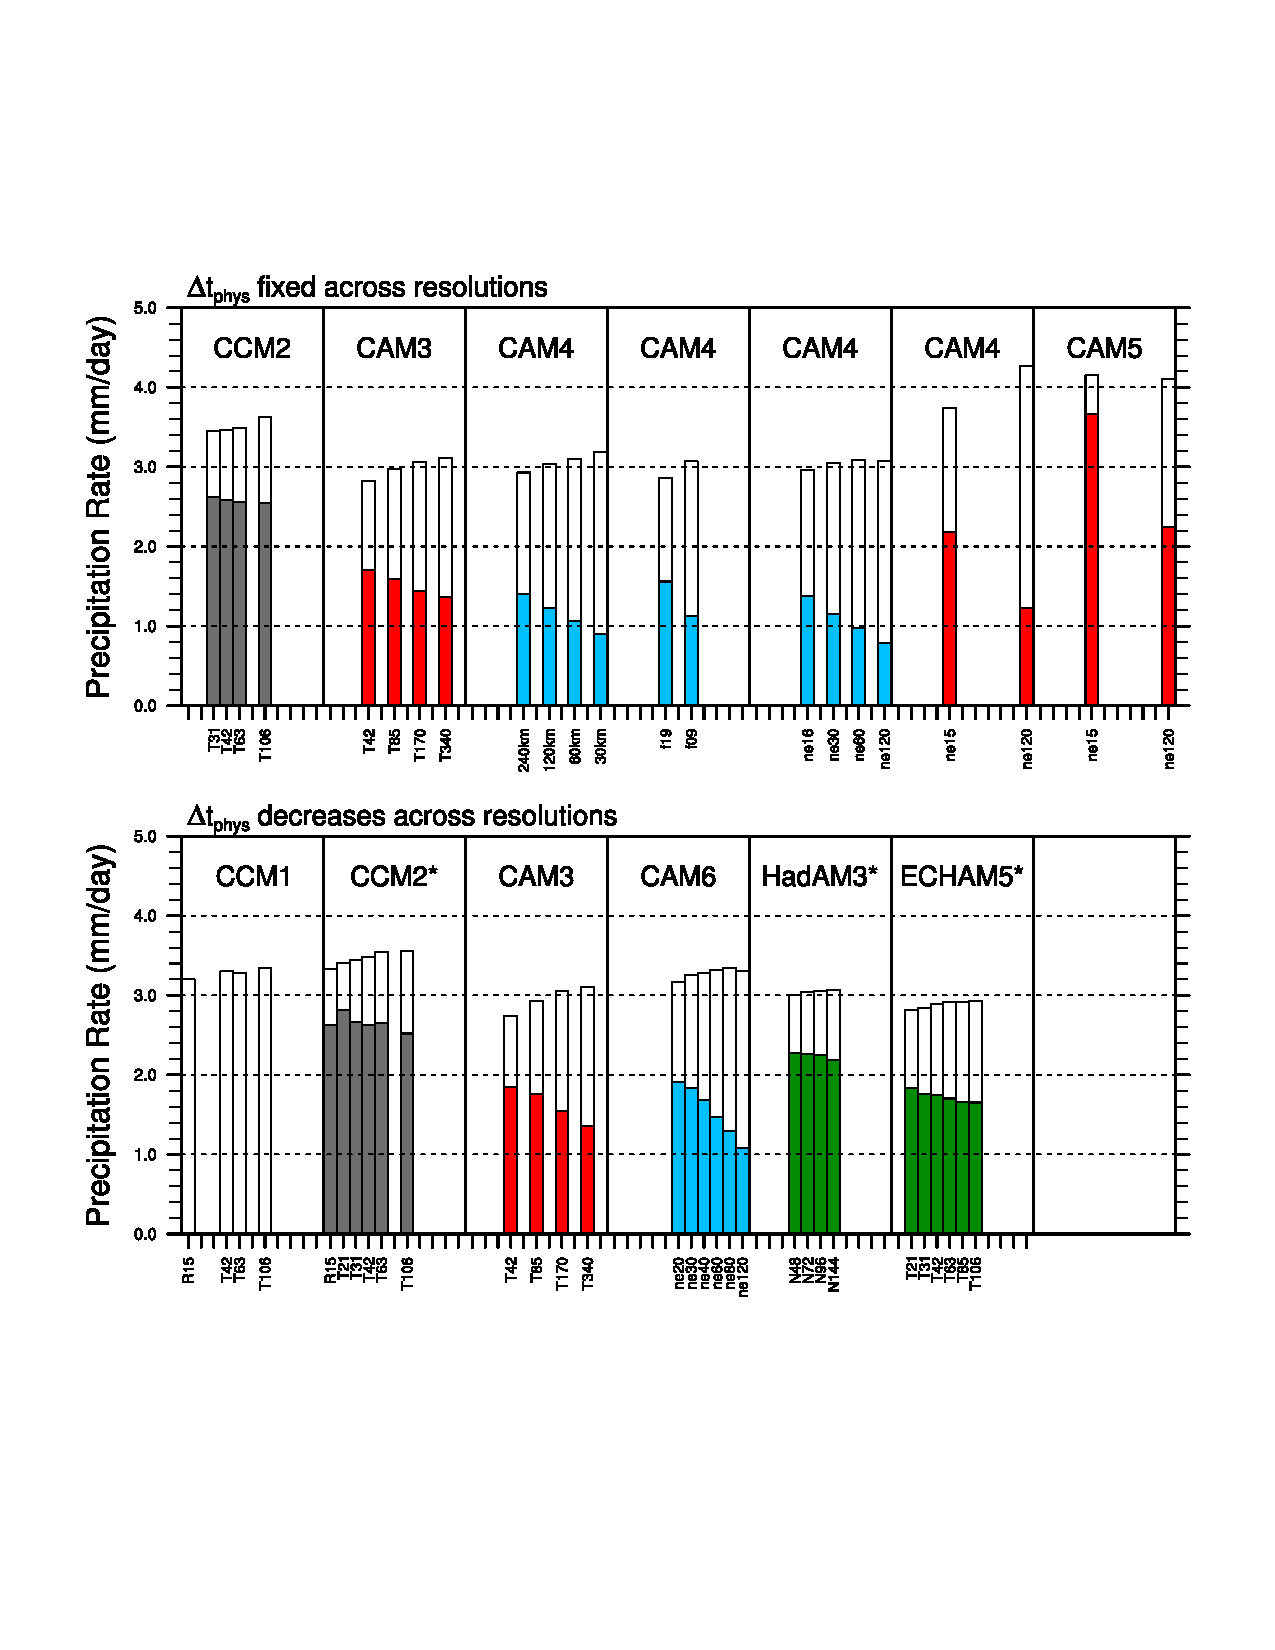
\includegraphics[width=20pc,angle=0]{figs/cam-history.pdf}\\
\end{center}
\caption{Bar-graph of the convective (solid) and grid-scale (white) climatological precipitation rates in prior CAM/CCM convergence studies. Each window contains a single convergence study, with identical x-axis; the approximate grid resolution. Colors indicate the model configuration; January ensemble (black) and aqua-planet configurations with SST profiles $QOBS$ (blue) and $CNTL$ (red) after \cite{NH2000ASL}. Studies included in this figure are \cite{KW1991JGR} (CCM1), \cite{WETAL1995CD} (CCM2), \cite{W2008TELLUS} (CAM3), \cite{RETAL2013JCLIM,ZetAl2014JCb,HR2017JCLIM} (CAM4), \cite{ZetAl2014JCb} (CAM5) and this study (CAM6). CCM2* refers to the modified parameter experiment of \cite{WETAL1995CD}, where parameters vary with resolution to reduce the dependence of cloud fraction on resolution.}
\label{fig:cam-history}
\end{figure}

In this study, a convergence experiment using CAM, version 6 (CAM6; \url{https://ncar.github.io/CAM/doc/build/html/users_guide/index.html}) is carried out and analyzed in detail. It is shown that the resolution sensitivity of vertical velocities are well described with $n=-1$ in equation~\eqref{eq:alpha}, provided $\Delta t_{phys}$ is defined in a way that avoids large truncation errors across resolutions. The reduction in convective precipitation rates with resolution in CAM6 is shown to result from the greater magnitude subsiding motion, creating a more stable atmosphere in which the criterion for parameterized convection occurs less often. The feedback of the resolved vertical motion on the physics indicates that the root cause of resolution sensitivity in CAM arises from the sensitivity of resolved dynamical modes to native grid resolution. Section 2 describes CAM6 and details the convergence experiment. Section 3 contains a thorough analysis of the CAM6 simulations and Section 4 provides some discussion and conclusions.

\section{Methods}

\subsection{Dynamical Core}

This study uses the spectral-element dynamical core option of Community Atmosphere Model \citep[CAM-SE;][]{DetAl2012IJHPCA}, coupled with a mass conserving, semi-Lagrangian advection method for accelerated multi-tracer transport \citep[CSLAM;][]{LTOUNGK2017MWR}, and dry-mass vertical coordinate with comprehensive treatment of moisture and energy \citep{LetAl2018JAMES}. The dry dynamics are solved using the high-order, momentum, mass and energy conserving spectral element method \citep{TF2010JCP}, with the elements defined by a cubed-sphere grid. The notation for the horizontal grid resolution is an `$ne$' followed by the number of elements making up an edge of one cubed-sphere face, e.g., $ne30$. Hyper-viscous $\nabla^{4}$ explicit numerical dissipation is applied to temperature, dry pressure thickness, rotational and divergent winds. CSLAM tracer transport uses a finite volume grid constructed from the cubed-sphere of elements, and contains the same degrees of freedom as the dry dynamics.

\subsection{Physical Parameterizations}

The physics are evaluated on the finite-volume CSLAM grid, and the tendencies mapped back to the spectral element grid. The coupled system, referred to as CAM-SE-CSLAM, conserves energy, mass and preserves linear correlations between two reactive species to within machine precision \citep{HL2018MWR}. A coarser physics grid, containing $\frac{5}{9}$ fewer degrees of freedom than the dynamical core grid is also available as part of the CAM-SE-CSLAM package \citep{HETAL2019JAMES}. This lower-resolution physics grid is used in this study, but only as a member of a perturbed parameter ensemble and not in the default convergence experiment. The dynamics time-step is subcycled within a longer physics time-step $\Delta t_{phys}$, and the temperature and momentum increments from the physics are divided by the number of subcycles and added to the dynamical core at the beginning of each subcycle. The full moisture increment from the physics is applied only at the start of the first subcycle to conserve tracer mass \citep[$ftype=2$ option in][]{LetAl2018JAMES}.

The simulations use the CAM6 physics package. The Cloud Layers Unified by Binormals \citep[CLUBB][]{GETAL2002JAS,BOG2013JCLIM} is an assumed PDF high-order closure model that handles shallow convection, planetary boundary layer mixing and cloud macrophysics. The macrophyiscs are coupled with a two-moment bulk cloud microphysics scheme with prognostic precipitation \citep{MG2}, and microphysics are coupled with a three mode Modular Aerosol Model \citep{MAM}. The combined macrophysics/microphysics routines generate grid-scale clouds with stratiform precipitation. Deep convection is parameterized using a quasi-equilibrium mass flux scheme \citep{ZM1995AO} and a dilute form of the convective available potential energy (CAPE) is computed to assess the convective trigger ($\geq 70$ J/kg), and for closing the mass fluxes in the cloud ensemble \citep{NRJ2008JC}. The deep convection scheme also parameterizes convective momentum transport \citep{RR2008JC}.

\subsection{Experimental Design}
 
The convergence experiment is performed in an aqua-planet configuration \citep{NH2000ASL,MWO2016JAMES}, an all ocean planet with fixed, zonally symmetric sea surface temperatures modeled after present day Earth \citep[$QOBS$ in][]{NH2000ASL}. The aqua-planets are in a perpetual equinox, and aerosols are largely absent from the simulations. Each simulation is ran for one simulated year. Six different horizontal grids are used in this study, which are provided in Table~\ref{tbl:table1}. The horizontal hyper-viscosity operators $\nu$ vary with resolution after \cite{HETAL2019JAMES}, also provided in Table~\ref{tbl:table1}. The values of $\nu$ are a factor 2.5 greater for divergence damping and are not shown. $\Delta t_{phys}$ is chosen to scale with resolution, in proportion to the grid spacing,
\begin{equation}
\Delta t_{phys} = \Delta t_{phys,0} \times \frac{n_{e,0}}{n_e}~s,\label{eq:dt-scale}
\end{equation}
where $\Delta t_{phys,0}$ is taken to be the standard $1800 s$ used in CAM-SE-CSLAM at the standard resolution, $n_{e,0} = ne30$ (equivalent to an average equatorial grid spacing $\Delta x = 111.2$km). This scaling was chosen to avoid large time-truncation errors in a rising moist bubble test \citep[Appendix A in][]{HETAL2019JAMES}, and it is understood that this choice of $\Delta t_{phys}$ will likely lead to greater resolution sensitivity \citep{W2008TELLUS}. The convective time-scale in the deep convection scheme is fixed at 3600 s in all simulations.
 
\section{Results}

 \begin{table}
 \caption{Experimental design and global means.}
 \centering
 \scriptsize
 \begin{tabular}{lcccccc}
   \hline
   Variable & $ne20$ & $ne30$ & $ne40$ & $ne60$ & $ne80$ & $ne120$ \\
   \hline
   $\nu$ ($m^4/s$) & $1.5 \times 10^{15}$ & $4.0 \times 10^{14}$ & $1.5 \times 10^{14}$ & $4.0 \times 10^{13}$  & $1.5 \times 10^{13}$ & $4.0 \times 10^{12}$\\
    $\Delta t_{phys}$ (s) & 2700 & 1800 & 1350 & 900 & 675 & 450 \\
   Total Cloud Fraction & 0.844 & 0.835 & 0.824 & 0.810 & 0.804 & 0.800 \\ 
   Total Precipitable Water (mm) & 23.31& 23.01 & 22.62 & 22.25 & 21.93 & 21.72 \\
   Convective Precipitation (mm/day) & 1.91 & 1.83 & 1.68 & 1.47 & 1.29 & 1.08 \\
   Stratiform Precipitation (mm/day) & 1.26 & 1.42 & 1.60 & 1.85 & 2.05 & 2.22 \\      
 \hline
 \end{tabular}
 \label{tbl:table1}
 \end{table}

Table~\ref{tbl:table6-1} provides a list of some relevant globally averaged metrics that are typically published in CAM-lineage convergence studies. Total precipitable water, total cloud fraction and deep convective precipitation rate decreases, while stratiform precipitation increases, monotonically with resolution. Resolution sensitivity in CAM6 is similar to all prior model versions within the models' lineage. 

The probability density function (PDF) of negative, or upward vertical pressure velocities $\omega$ in the aqua-planets is shown in Figure~\ref{fig:2pdf}a. The magnitude of upward $\omega$ increases in a monotonic way with resolution, with positive, or downward $\omega$ behaving similarly (not shown). The PDF's may be scaled to the high-resolution $ne120$ resolution through $P(\omega)_s = \alpha P (\omega / \alpha)$, where $\alpha$ is the scale factor equation~\ref{eq:eq6-1}. In general, the scaled PDF's all line up on top of the high-resolution reference (Figure~\ref{fig:2pdf}b); equation~\ref{eq:eq6-1} explains the variation in vertical velocity across resolutions to first order. 

\begin{figure}[t]
\begin{center}
\noindent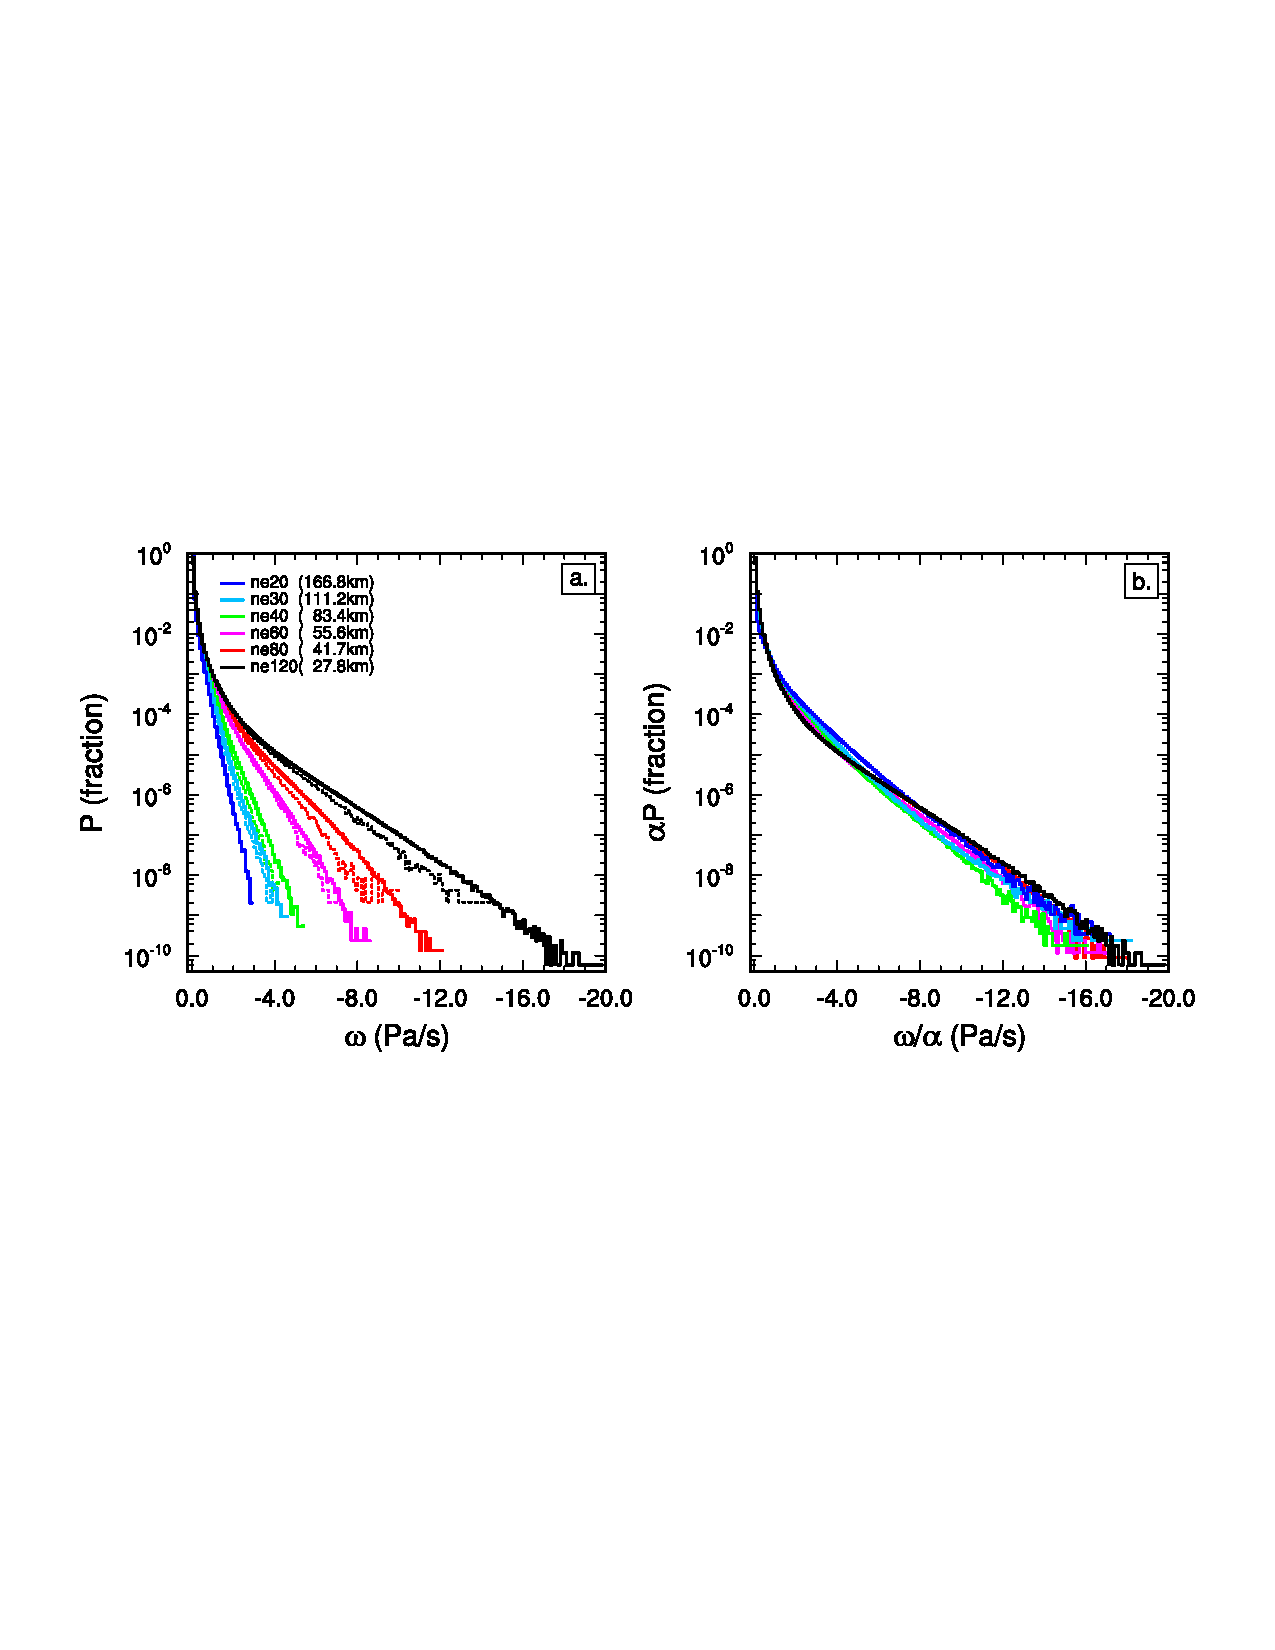
\includegraphics[width=20pc,angle=0]{figs/temp_2pdf.pdf}\\
\end{center}
\caption{Probability density distribution of the upward vertical pressure velocities $\omega$ computed everywhere in the model from 1 year of 6-hourly data (a) raw values (b) scaled to the $ne120$ resolution using $P(\omega)_s = \alpha P (\omega / \alpha)$, where $\alpha$ is from equation~\ref{eq:eq6-1}.}
\label{fig:2pdf}
\end{figure}

Changes to the time-mean vertical velocity field can be understood through decomposing the global mean $\omega$ into upward and downward components,
\begin{equation}
\overline{\langle \omega \rangle} = \overline{\langle f_{u} \rangle} \, \overline{\langle \omega_{u} \rangle} + \overline{\langle f_{d} \rangle} \, \overline{\langle \omega_{d} \rangle}, \label{eq:eq6-2}
\end{equation}
where $\langle f_x \rangle$ and $\langle \omega_x \rangle$ refers to the vertical mass fraction and contribution to mass weighted vertical mean $\omega$, respectively, subscript $u$ refers to upward motion and $d$, downward motion; overbars indicate time-mean.

The components of equation~\ref{eq:eq6-2} are shown in Figure~\ref{fig:8panel}a,b,e,f for the six aqua-planet simulations. The magnitude of both $\overline{\langle \omega_{u} \rangle}$ and $\overline{\langle \omega_{d} \rangle}$ increase monotonically with resolution, the upward component increasing more than the downward component. In contrast, $\overline{\langle f_{u} \rangle}$ decreases with resolution while $\overline{\langle f_{d} \rangle}$ increases, although in both cases there is a reversal in this trend in the highest resolution simulation, $ne120$. Note that the magnitude of the change in $\overline{\langle f_{u} \rangle}$ and $\overline{\langle f_{d} \rangle}$ is small, a range of about $0.015$ across all simulations. Figure~\ref{fig:8panel}c,g shows that the products  $\overline{\langle f_{u} \rangle} \, \overline{\langle \omega_{u} \rangle}$ and $\overline{\langle f_{d} \rangle} \, \overline{\langle \omega_{d} \rangle}$ are equal and opposite, which is a requirement of mass conservation in the model and a convenient check of the calculation. Besides the six aqua-planets described in Section 6.2, 23 additional year-long aqua-planet experiments were carried out at various resolutions, with modified parameters in the dynamical core and the physics. The spread in the components of equation~\ref{eq:eq6-2} in the simulations with perturbed parameters is relatively large for $\overline{\langle f_{x} \rangle}$, compared with $\overline{\langle \omega_{x} \rangle}$.

\begin{figure}[t]
\begin{center}
\noindent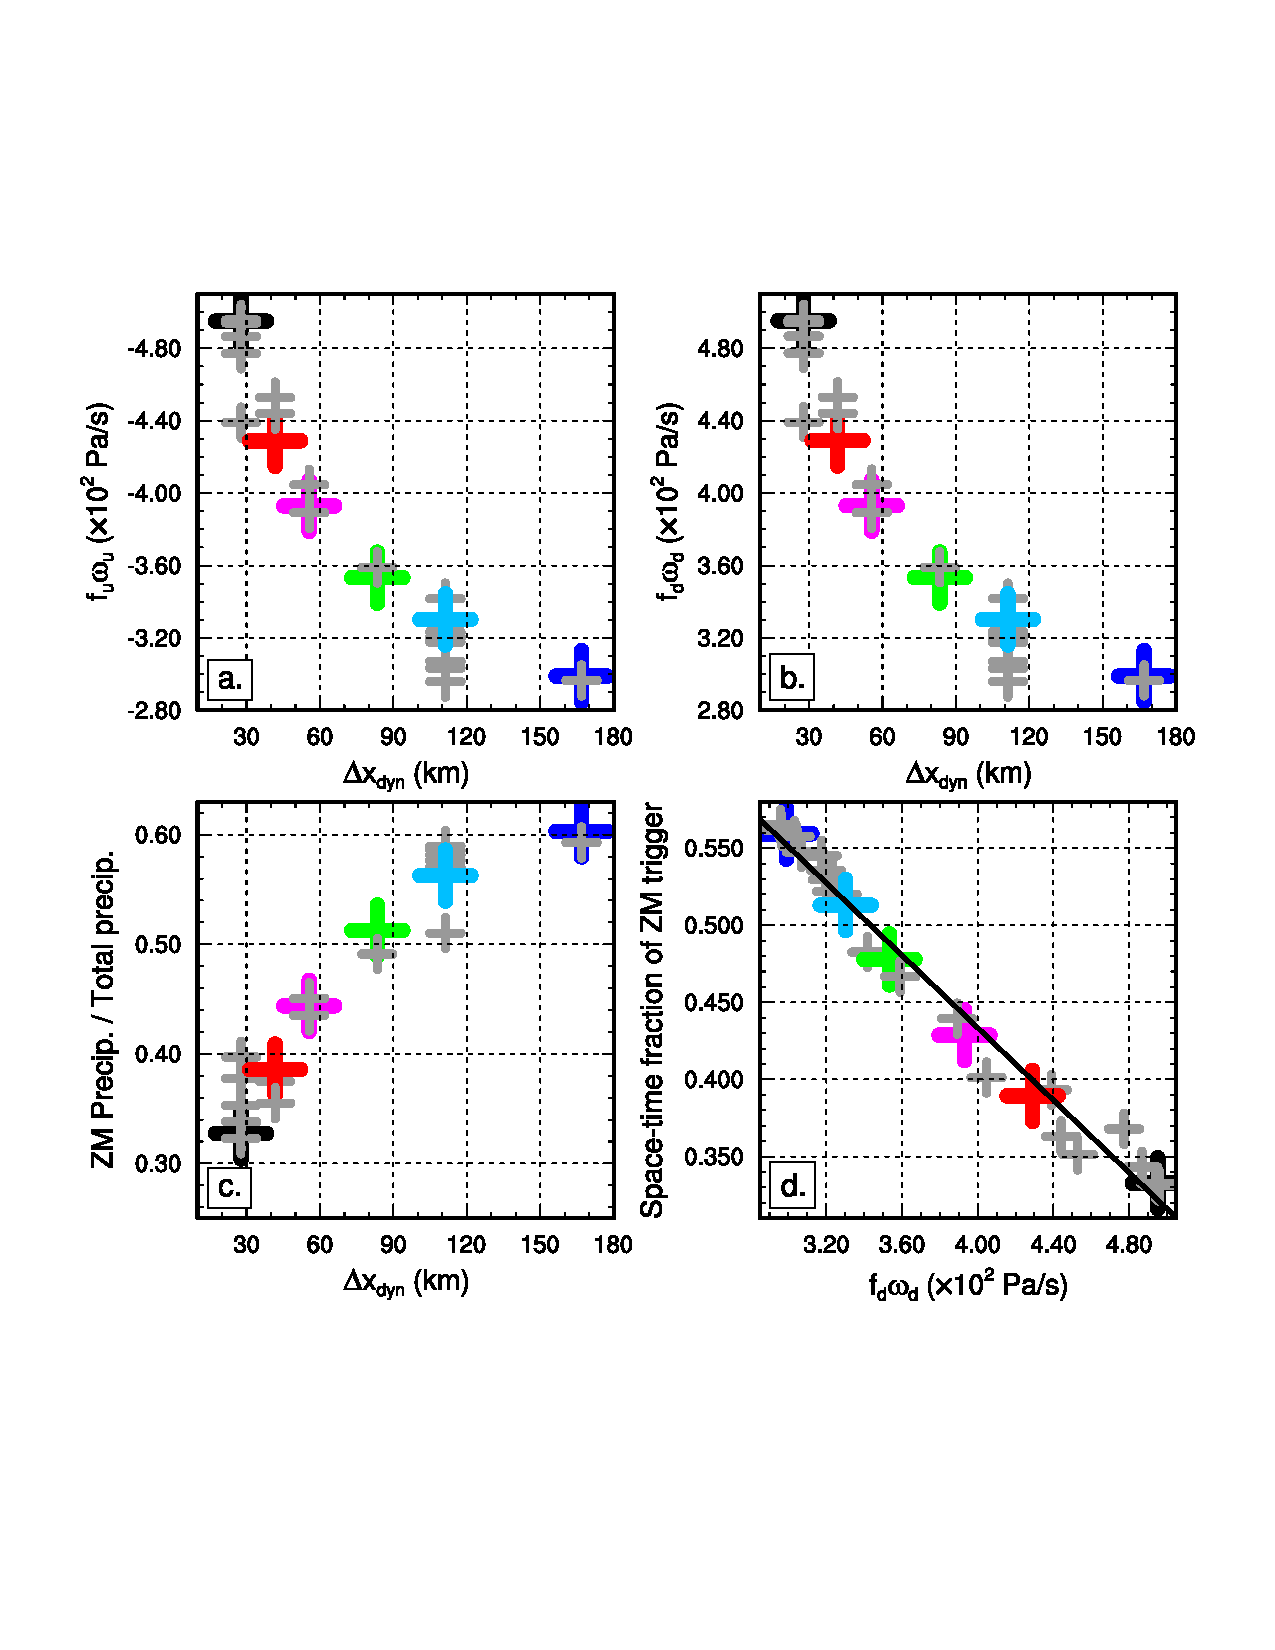
\includegraphics[width=20pc,angle=0]{figs/temp_diags_4panel.pdf}\\
\end{center}
\caption{(a,b,c,e,f,g) Components of the global mean vertical pressure velocity $\overline{\langle \omega \rangle}$ (d) ratio of global mean ZM precipitation rate to the total precipitation rate versus grid spacing $\Delta x$ and (e) scatter plot of $\overline{\langle f_{d} \rangle} \, \overline{\langle \omega_{d} \rangle}$ and FREQZM, and the fitted linear regression which has a Pearson's R-value = 0.99. (a) $\overline{\langle \omega_{u} \rangle}$ (b) $\overline{\langle f_{u} \rangle}$ (c) $\overline{\langle f_{u} \rangle} \, \overline{\langle \omega_{u} \rangle}$ (e) $\overline{\langle \omega_{d} \rangle}$ (f) $ \overline{\langle f_{d} \rangle}$ (g) $\overline{\langle f_{d} \rangle} \, \overline{\langle \omega_{d} \rangle}$. Colors are as in Figure~\ref{fig:2pdf}. Grey crosses are for the perturbed parameter runs.}
\label{fig:8panel}
\end{figure}

The reduction in the \cite{ZM1995AO} deep convective precipitation rate (hereafter referred to as the {\em{ZM precipitation}}) is depicted in Figure~\ref{fig:8panel}d, which shows the global mean fraction of total precipitation arising from ZM precipitation decreasing from about $0.60$ at low resolution ($ne20$) to about $0.32$ at high resolution ($ne120$). This reduction in ZM precipitation manifest through triggering less frequently (not shown). The space-time fraction the ZM precipitation scheme is triggered (hereafter referred to as the {\em{FREQZM}}) is highly negatively correlated with $\overline{\langle f_{d} \rangle} \, \overline{\langle \omega_{d} \rangle}$ in the 29 simulations (Pearson's R-value = 0.99; Figure~\ref{fig:8panel}h), more then with any individual component of equation~\ref{eq:eq6-2}.

Figure~\ref{fig:vomg}a,b shows the time mean zonal mean $\langle f_{d} \rangle \langle \omega_{d} \rangle$ and FREQZM. $\langle f_{d} \rangle \langle \omega_{d} \rangle$ is smallest in the deep tropics (equatorward of about $10^{\circ}$), increasing sharply poleward throughout the subtropics and then begins to decrease in the middle latitudes ($\geq 40^{\circ}$) and conitnuing into the polar regions. FREQZM is largely opposite of $\langle f_{d} \rangle \langle \omega_{d} \rangle$; where greater subsiding motion occurs FREQZM is small, except in the mid-latitude region between $30^{\circ}$ and $60^{\circ}$ where the spatial variations are quite different. The resolution sensitivity of these two quantities has no zonal dependence; $\langle f_{d} \rangle \langle \omega_{d} \rangle$ increases and FREQZM decreases just about everywhere with resolution, in similar proportions.

\begin{figure}[t]
\begin{center}
\noindent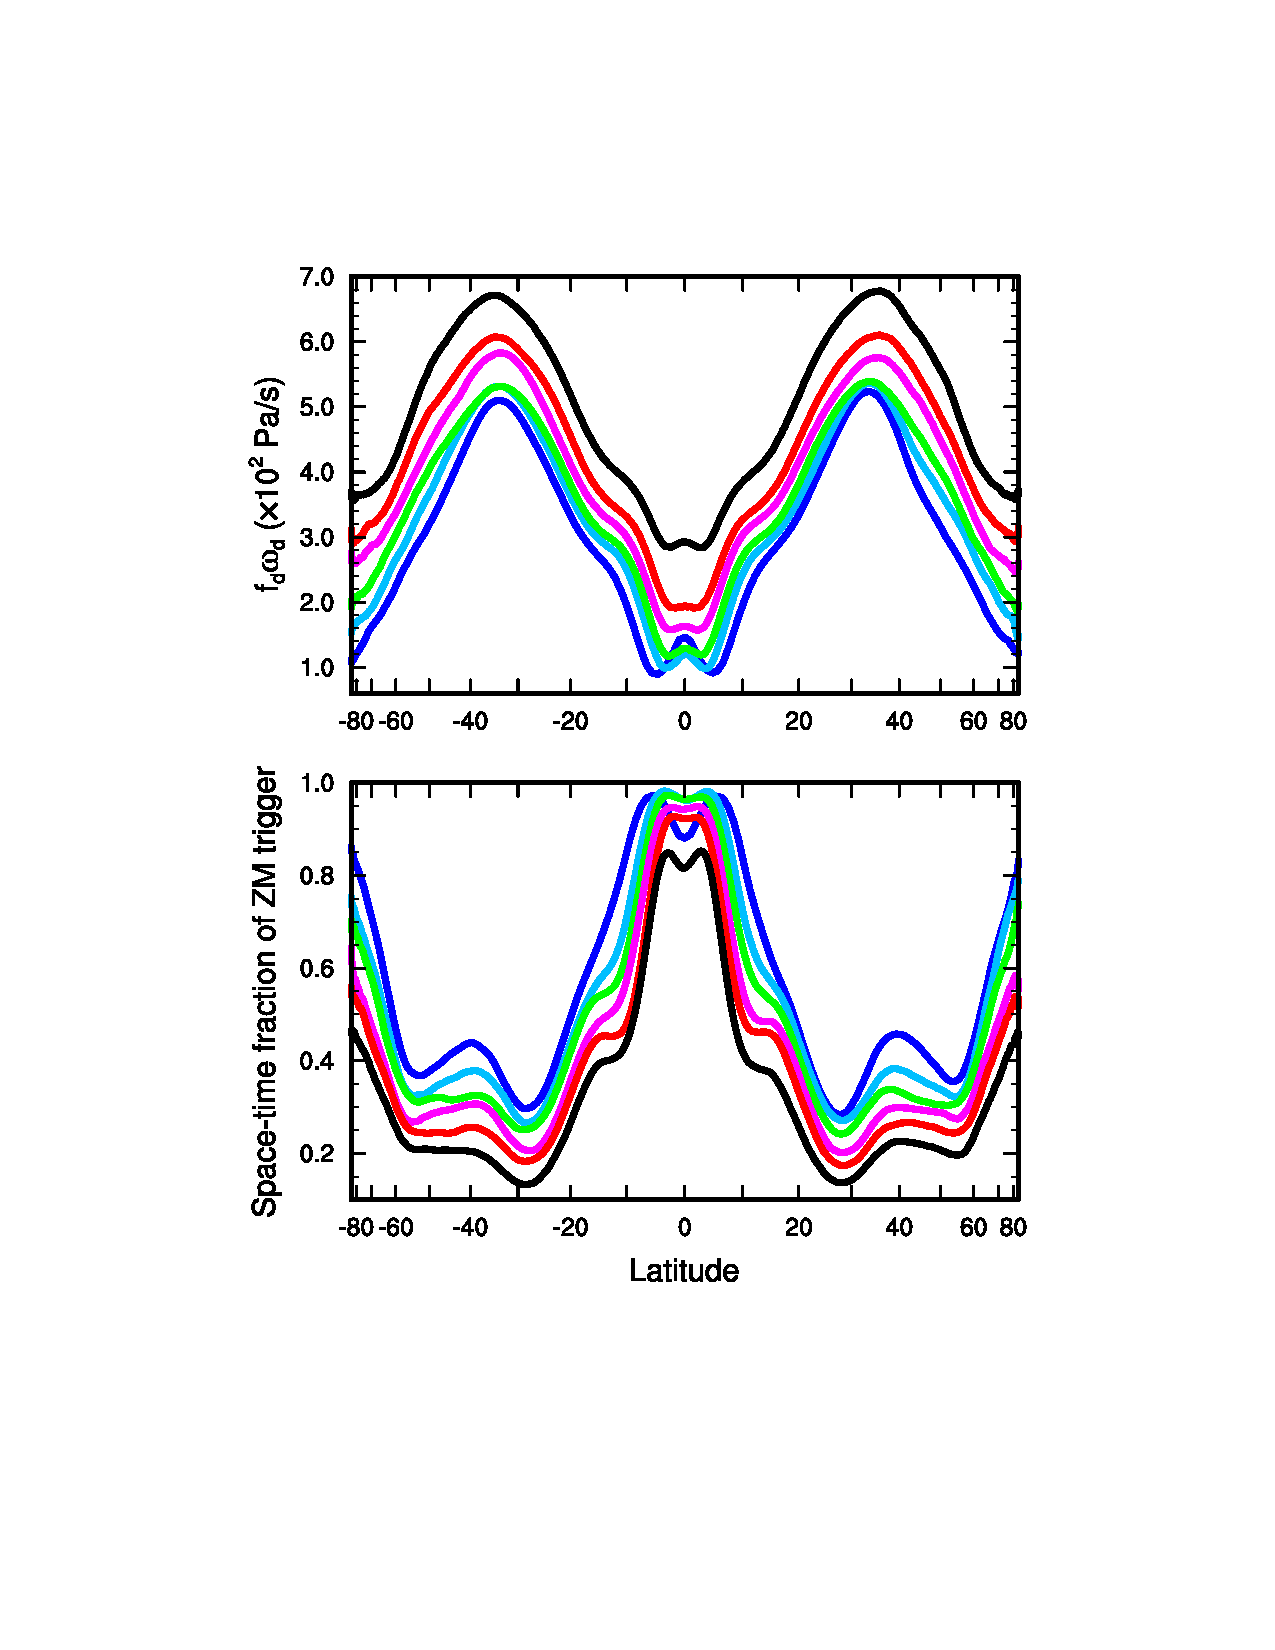
\includegraphics[width=17pc,angle=0]{figs/temp_zonal_fracd*vomgd.pdf}\\
\end{center}
\caption{Time mean zonal mean (a) $\langle f_{d} \rangle \langle \omega_{d} \rangle$, (b) FREQZM. Colors are as in Figure~\ref{fig:2pdf}.}
\label{fig:vomg}
\end{figure}

The ZM trigger uses a dilute form of CAPE, which is consistent with the negative relation between $\overline{\langle f_{d} \rangle} \, \overline{\langle \omega_{d} \rangle}$ and FREQZM in space, and across resolutions. In the classical, non-dilute case, CAPE can be seperated into two components \citep{Z2002JGR}; instability due to the thermodynamic state of parcels in the boundary layer and the instability generated through advection of dry static energy and moisture by the environment, i.e., the resolved flow. The latter term generally contributes positively to CAPE in regions of ascent and negatively in regions of subsidence \citep{SZ2018JCLIM}, consistent with the negative correlation of $\langle f_{d} \rangle \langle \omega_{d} \rangle$ in space, and across resolutions.

\begin{figure}[t]
\begin{center}
\noindent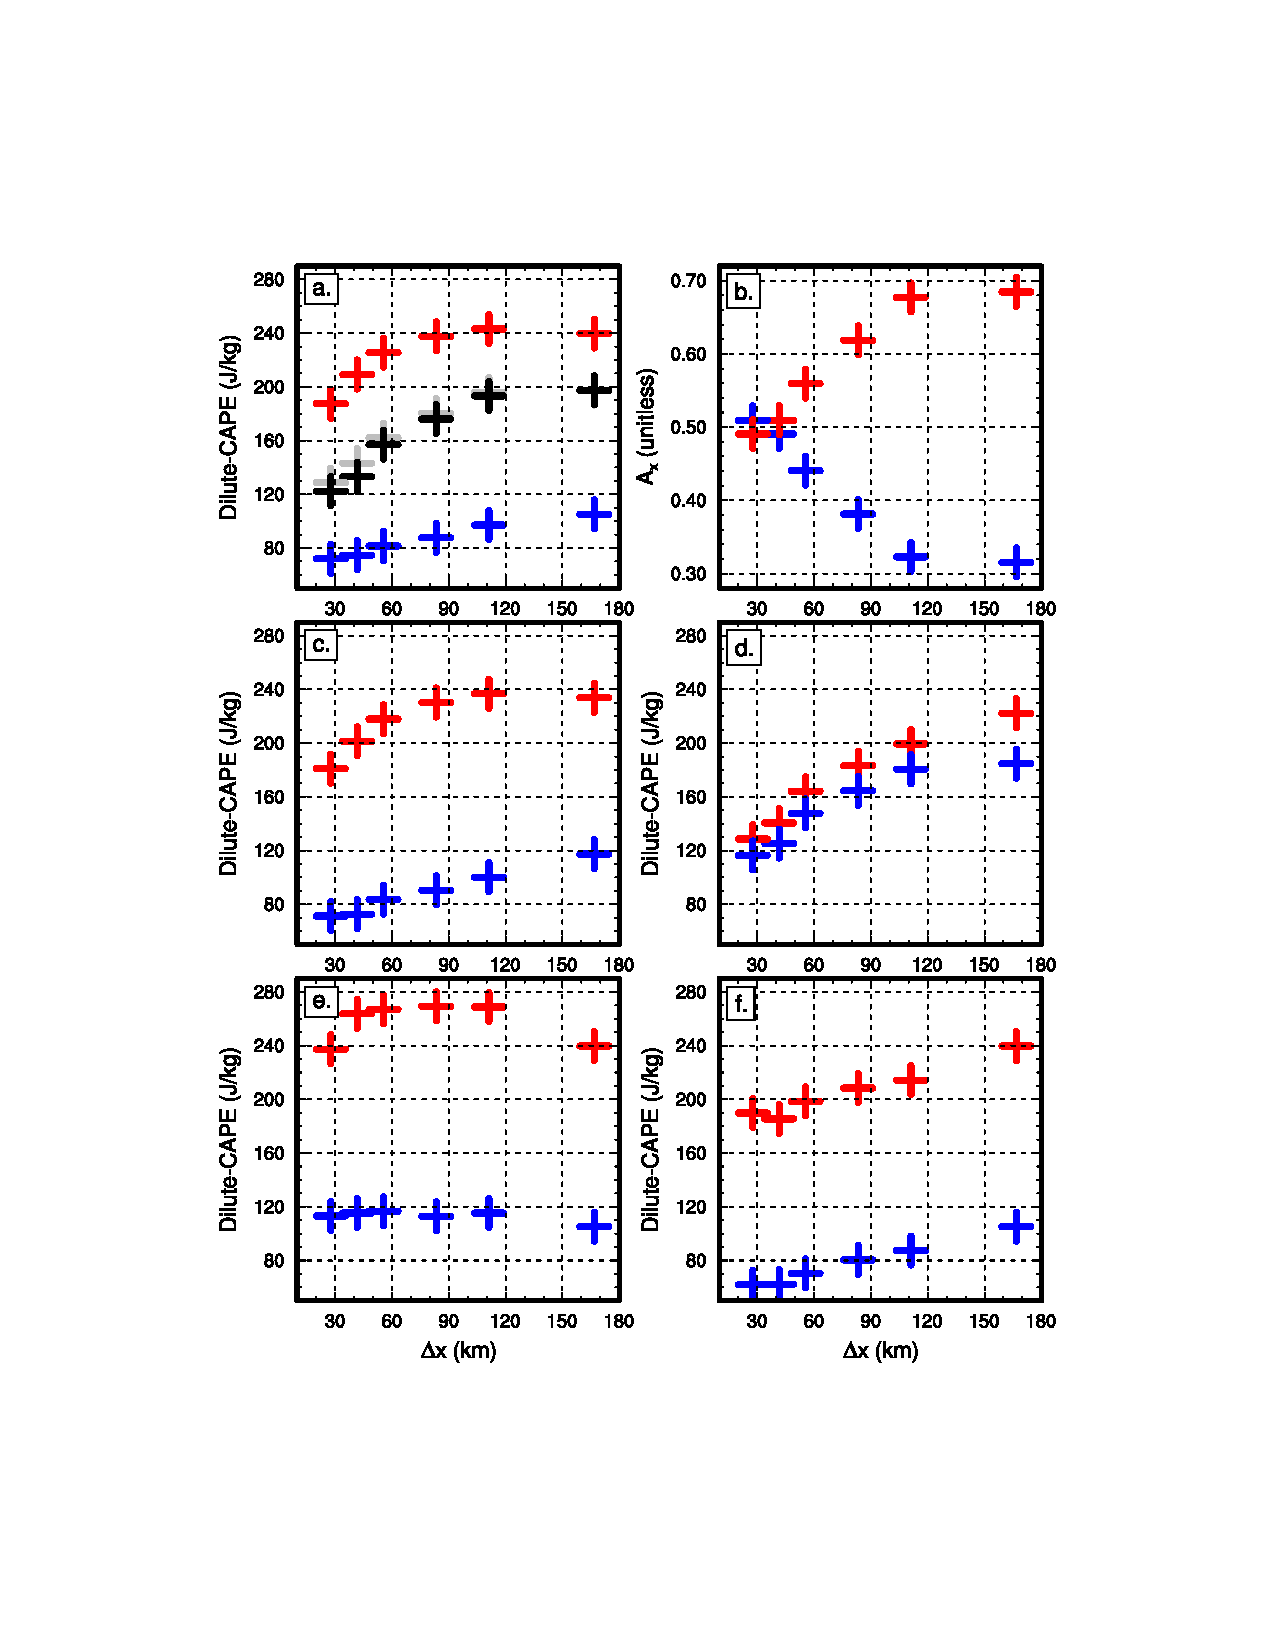
\includegraphics[width=20pc,angle=0]{figs/temp_cape.pdf}\\
\end{center}
\caption{(a) time mean fraction of the deep tropics in the simulations with upward $\langle \omega \rangle$ (red) and downward $\langle \omega \rangle$ (blue), (b) CAPE computed from the mean temperature and moisture profiles of upward regions and downward regions. Black is for CAPE computed from the mean temperature and moisture profiles for the entire deep tropics, grey is the approximate discussed in the text.}
\label{fig:cape}
\end{figure}

To further support a negative relation between subsiding motion and CAPE, temperature and moisture profiles are collected from the deep tropics in the simulations, and conditionally sampled depending on whether $\langle \omega \rangle$ is positive or negative, indicating predominantly subsiding or ascending grid columns. The mean temperature and moisture profiles of subsiding and ascending regions are then used to compute the dilute-CAPE used by the ZM scheme, offline. Figure~\ref{fig:cape}b indicates that the mean profile of ascending regions are associated with large values of CAPE ($>170$ J/kg), and low values in subsiding regions ($<110$ J/kg). The mean profiles of subsiding regions have an anomalous warming layer in the $600-800$ hPa layer and an anomalous moisture deficit throughout the entire column, relative to the non-conditionally sampled mean (not shown). Figure~\ref{fig:cape}a shows that fractional area of air columns in the deep tropics that are predominantly subsiding (ascending) changes drastically with resolution, from $0.32$ ($0.68$) in the $ne20$ ($\Delta x = 166.8$ km) run, and monotonically increasing (decreasing) with resolution to $0.51$ ($0.49$) in the $ne120$ ($\Delta x = 27.8$ km) run. Interestingly, the sum of the product of the fractional areas with their corresponding CAPE values gives approximately the same CAPE values computed from the non-conditionally sampled mean temperature and moisture profiles (Figure~\ref{fig:cape}b). This provides strong evidence that CAPE values in the deep tropics are decreasing with resolution because a larger (smaller) fraction of the deep tropics are made up of subsiding (ascending) grid columns with resolution.

\begin{figure}[t]
\begin{center}
\noindent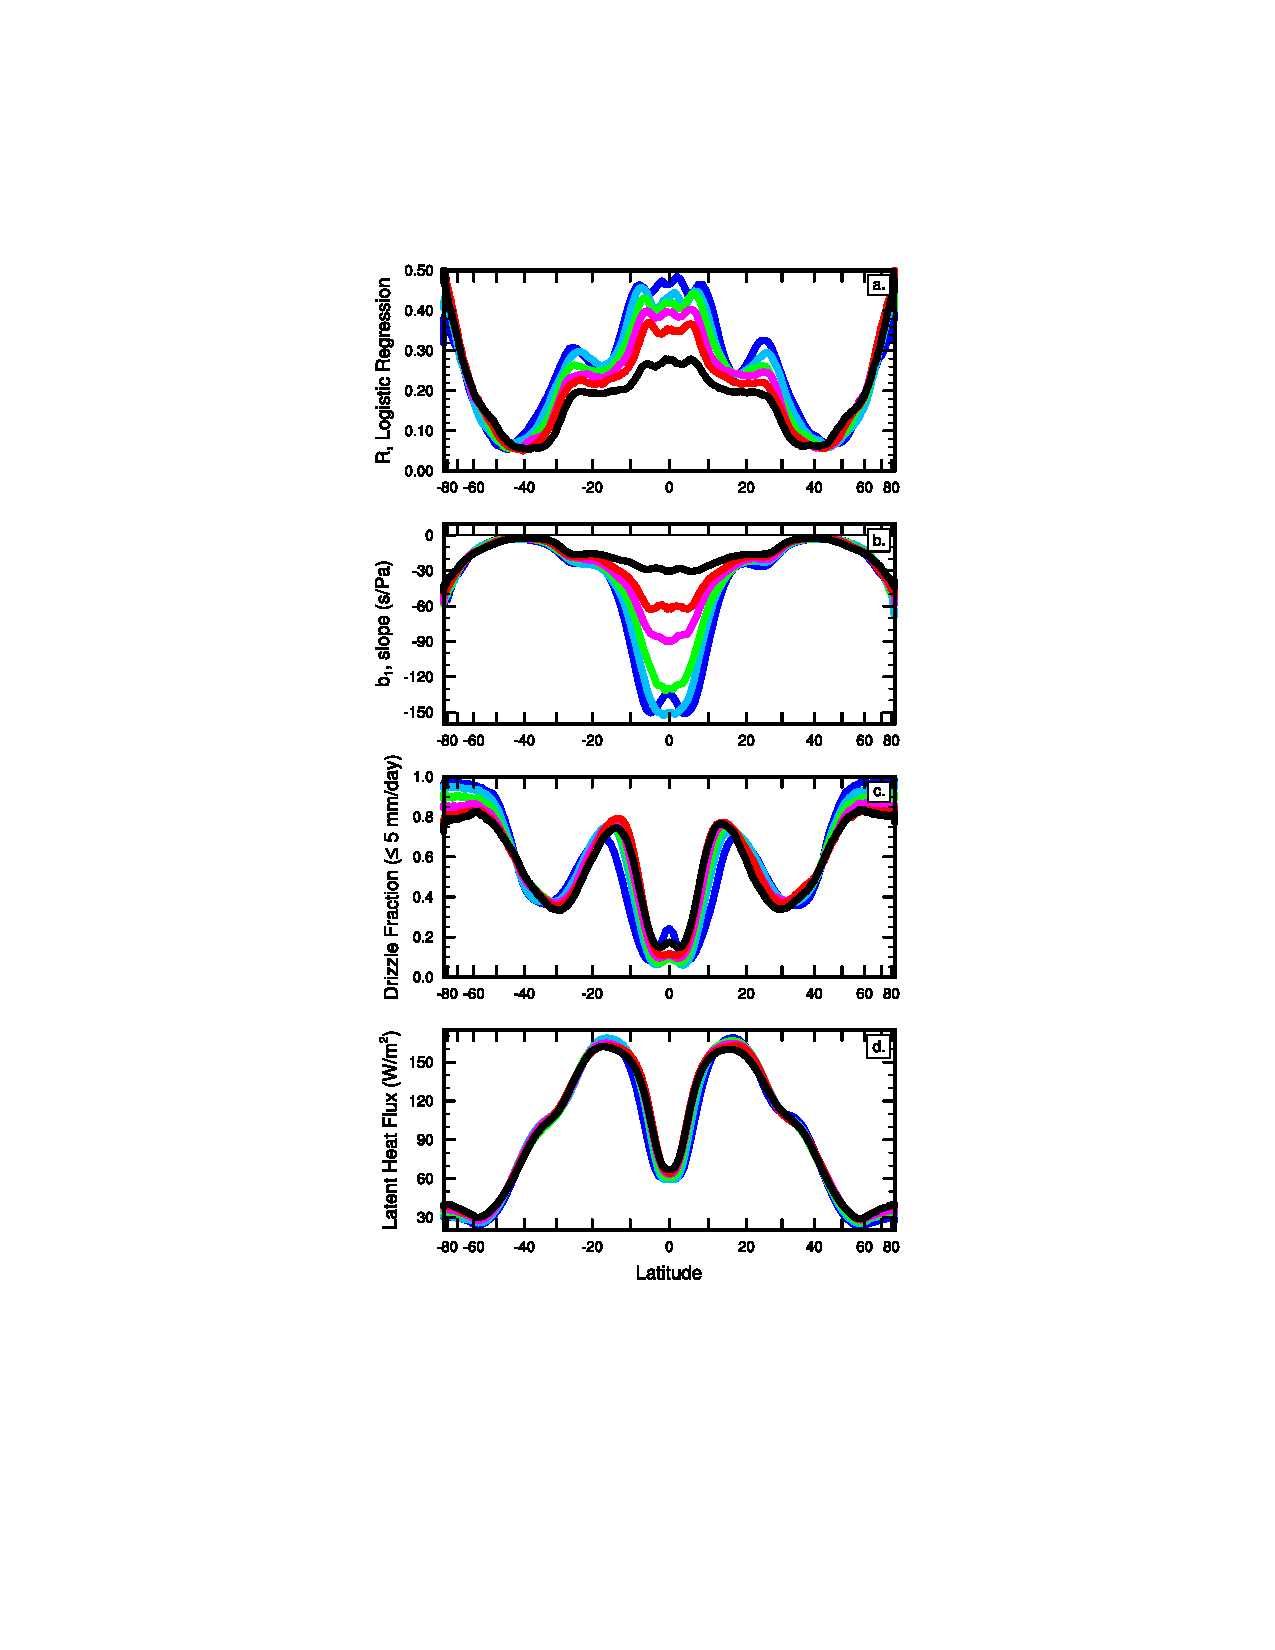
\includegraphics[width=14pc,angle=0]{figs/temp_zonal_4reg_dwn.pdf}\\
\end{center}
\caption{Zonal mean (a) R-values and (b) sensitivity parameter in the logistic regression, (c) drizzle fraction, (d) time mean surface latent heat fluxes. Colors are as in Figure~\ref{fig:2pdf}.}
\label{fig:4reg}
\end{figure}

To understand how the relationship between subsiding motion and the trigger in the ZM scheme manifests within the simulations themselves, a logistic regression is performed for each grid column in the simulations. Logistic regression uses an iterative method to fit a continuous variable predictor, $x$ to a binary predictand $p$ \citep{WILKSBOOK},
\begin{equation}
p = \frac{exp{[b_0 + b_1 x]}}{1 + exp{[b_0 + b_1 x]}}, \label{eq:eq6-3}
\end{equation}
where $b_0$ and $b_1$ are the shape parameters of the exponential. The predictor is chosen as the instantaneous $\langle f_{d} \rangle \langle \omega_{d} \rangle$ of a grid column, and the predictand is whether or not the ZM scheme is active, $1$ for yes and $0$ for no. Since the aqua-planets have zonally symmetric boundary conditions, there is a zonally varying structure in the goodness of fit (R-value) and parameter $b_1$ (hereafter referred to as the sensitivity parameter). Figure~\ref{fig:4reg}a shows the zonal mean R-values indicates the goodness of fit is greatest in the deep tropics. Figure~\ref{fig:4reg}d shows the time mean zonal mean latent heat flux in the simulations, which is expected to contribute positively to CAPE through the component associated with the thermodynamic state of boundary layer parcels. In the deep tropics, the latent heat flux is small, and the sensitivity parameter is large and negative (Figure~\ref{fig:4reg}b), indicating that subsiding motion is successfully depressing CAPE, and the activity of the ZM scheme in that region.

Poleward of $10^{\circ}$, the R-value decreases to a local minimum between $15^{\circ} - 20^{\circ}$ latitude, and the magnitude of the sensitivity parameter steeply declines. Even though the subsiding motion is increasing polewards of $10^{\circ}$, this motion is less effective in depressing the convection scheme. The local minimum in the R-value corresponds with a local maximum in the latent heat fluxes, indicating that the subsiding motion is less skillful a predictor of the ZM scheme when the boundary layer is being driven unstable by large surface latent heat fluxes. The CAPE values in the $10^{\circ} - 15^{\circ}$ latitude region are likely to be small, since the ZM precipitation rate consists primarily of drizzle (Figure~\ref{fig:4reg}c). The predominance of drizzle in this region is probably a result of the large subsiding motion (Figure~\ref{fig:vomg}) constraining CAPE from becoming too large. AGCMs are known to suffer from an excess drizzle bias in precisely this approximate region \citep{D2006JCLIM}, and this analysis indicates that this bias is due to the use of a CAPE trigger function. In the $30^{\circ} - 60^{\circ}$ latitude region the shape parameter reaches it's global minimum and then begins to increase in the polar regions. This is consistent with lack of spatial correspondence between $\langle f_{d} \rangle \langle \omega_{d} \rangle$ and FREQZM in the mid-latitudes, and the reemergence of this correspondence in the polar regions (Figure~\ref{fig:vomg}).

The sensitivity parameter becomes less negative in the deep tropics with resolution, likely due to the greater magnitude $\langle f_{d} \rangle \langle \omega_{d} \rangle$ in that region with resolution, which requires a lower sensitivity parameter to predict the binary of whether the ZM scheme is active. The R-values generally decrease with resolution indicating that there is degradation in the relationship with resolution. All values shown are statistically significant at the $95\%$ level using a log-likelihood test \citep{WILKSBOOK}.
 
\section{Conclusions}

A convergence study is carried out in order to unravel the relationships between grid-scale clouds, parameterized convection and resolution sensitivity in an aqua-planet configuration of the Community Atmosphere Model (CAM) with version 6 physics (CAM6), the spectral-element dynamical core coupled to the Conservative Semi-Lagrangian Advection Method for advection of tracers and dry-mass vertical coordinate (CAM-SE-CSLAM). Common with just about all versions in the CAM-lineage, total cloud fraction, total precipitable water and convective precipitation decrease with resolution, while stratiform precipitation increases with resolution. The magnitude of vertical velocities everywhere in the model increase, and scale like the inverse of the grid spacing $\Delta x^{-1}$. The climatological area of regions of ascent decrease with resolution, the area of subsiding motion increases.

 The mass weighted vertical mean of downward vertical pressure velocities ($\langle f_{d} \rangle \langle \omega_{d} \rangle$) is highly negatively correlated with the frequency the \cite{ZM1995AO} deep convection scheme is triggered (FREQZM). The correlation of the climatological quantities is linear using 29 simulations containing a large range of grid resolutions, and has a goodness of fit Pearson's R-value of 0.99. A logistic regression between $\langle f_{d} \rangle \langle \omega_{d} \rangle$ and FREQZM was performed at each grid column in the simulations, and indicates that $\langle f_{d} \rangle \langle \omega_{d} \rangle$ is skillful at predicting FREQZM, with greater downward motion leading to less frequent convective triggering. This relationship is particularly strong in the deep tropics.
 
The \cite{ZM1995AO} deep convection scheme (ZM scheme) uses a Convective Available Potential Energy (CAPE) threshold as the convective trigger, and the high negative correlation between subsiding motion and the trigger is consistent with the dependence of CAPE on vertical advection of dry static energy and moisture \citep{Z2002JGR}. The precipitation rates in the $15^{\circ} - 20^{\circ}$ latitude region consist primarily of drizzle from the ZM scheme. The convective trigger is weakly correlated with rather strong subsiding motion in this region, but the latent heat fluxes into the boundary layer are at a global maximum. It is suggested that the downward motion is opposing the generation of CAPE by the latent heat fluxes of this region, but due to the overwhelming magnitude of the latent heat fluxes, cannot depress CAPE below the trigger threshold. The resultant CAPE values are small and ZM scheme produces drizzle most of the time. The excess simulation of drizzle in climate models is a known model bias \citep{D2006JCLIM}, and it is suggested here that this bias arises from the use of CAPE as the sole criterion for convective triggering.

The conclusion of this study builds on previous work \citep[][Chapter~\ref{sec:chapter5}]{HR2017JCLIM,HR2018JAMES}, and it is of the following relationships between parameterized convection, grid-scale clouds and resolution sensitivity in CAM. When the ZM scheme is triggered, it moistens the middle-to-upper troposphere through detrainment \citep{ZM1995AO}, moisture which is then condensed by the stratiform cloud scheme to produce grid-scale clouds. The buoyancy produced by grid-scale clouds leads to large magnitude upward motion by the dynamical core, and to conserve mass, downward motion radiating away from the grid-scale clouds as horizontally propagating gravity waves. The grid-scale clouds are grid-limited; their horizontal size is set by the effective resolution of the model. The vertical velocities associated with the buoyancy of stratiform clouds are inversely proportional to their horizontal extent, and therefore scale like $\Delta x^{-1}$. Due to the greater efficiency of vertical mass transport with increasing resolution, the area of ascending motion decreases with resolution. The area and magnitude of the subsiding regions increase with resolution in order to conserve mass, which has the effect of stabilizing and drying the atmosphere with increasing resolution. The ZM scheme, with its stability dependent CAPE trigger, responds through becoming less active with increasing resolution.


\ack This class file was developed by Sunrise Setting Ltd,
Paignton, Devon, UK. Website:\\
\href{http://www.sunrise-setting.co.uk}{\texttt{www.sunrise-setting.co.uk}}

\bibliographystyle{wileyqj}
\bibliography{bib}
\end{document}
